{$\space$\par}
\vspace{0.5cm}
\justifying
\section*{{\bfseries \LARGE Questão 4 -} {\bfseries \large  Compare a densidade das notas obtidas pelos alunos de 2024 com as de 2025 em uma figura com 6 paineis, um para cada nota. As distribuições são estatisticamente similares entre os alunos de cada ano?.}}

\vspace{0.2cm}

\textcolor{red}{Se buscamos verificar a similaridade estatística entre as distribuições de cada ano, precisamos de testes estatísticos que nos permitam realizar afirmações. Nessa sitaução, utilizei 4 testes: t-test, F-test, KS-test, Wilcox-test. A escolha dos testes foi feita de maneira que seja possível testes diferentes características das amostras. Além disso, decidir fazer um teste utilizando a MANOVA, ou seja, considerando a mediana de todas as dimensões ao mesmo tempo e obtive um valor p de: 0.49}

\begin{lstlisting}
    par(mfcol = c(3, 2)) 
    
    colors = c('blue', 'red')
    for (i in 2:7) {  
      values_1 = astro[astro$ano == 2025, i]
      values_2 = astro[astro$ano == 2024, i]
    
      # Tests
      t_test = t.test(values_1, values_2)
      f_test = var.test(values_1, values_2)
      ks_test = ks.test(values_1, values_2)
      wil = wilcox.test(values_1, values_2, exact = FALSE)
    
      # Plot
      plot(density(values_1), col = colors[1], xlab = 'Pontuação',
           main = colnames(astro)[i], ylim = c(0, max(density(values_1)$y,
            density(values_2)$y) * 1.2))
      lines(density(values_2), col = colors[2])
    
      # Add text
      text_x = median(median(values_1),median(values_2)) *0.8
      y_start = 0.008
    
      text(text_x, y_start*0.9,     paste("t: ", round(t_test$p.value, 3),
      "\nF: ", round(f_test$p.value, 3),
      "\nKS: ", round(ks_test$p.value, 3),
      "\nWil: ", round(wil$p.value, 3)), pos = 3)
    }
    
    legend('topleft', legend = c(2025, 2024), col = colors, lty = 1, bty = 'n', 
    cex = 1.2)
    # MANOVA
    man_test = manova(as.matrix(astro[,2:7]) ~ astro$ano)
    cat("\nMANOVA teste para todas as áreas:\n")
    print(summary(man_test))
\end{lstlisting}

\begin{figure}[h]
    \centering
    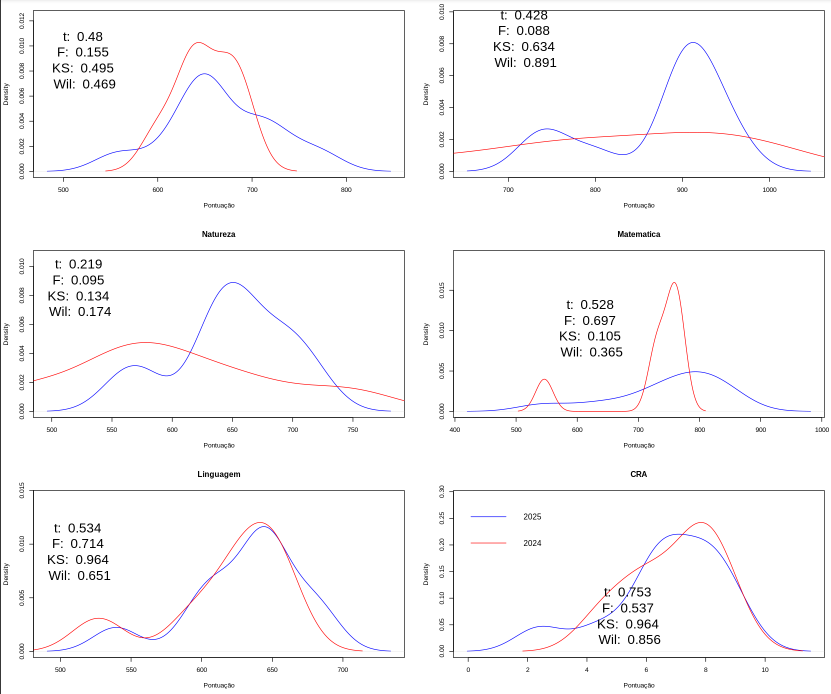
\includegraphics[width=1\linewidth]{Figuras/grades.png}
    \caption{Distribuição da notas dos alunos da astronomia classificados por ano de ingresso junto com o valor p dos 4 testes estatísticos escolhidos para a análise.}
    \label{grades}
\end{figure}

\vspace{8em}

\textcolor{red}{Ao olhar o resultado de diferentes testes na figura \ref{grades}, não podemos afirmar que as distribuições são de diferentes populações. Portanto, pode-se dizer que são estatisticamente similares.}
